\documentclass[a4paper]{article}

\usepackage{fullpage} % Package to use full page
\usepackage{parskip} % Package to tweak paragraph skipping
\usepackage{tikz} % Package for drawing
\usepackage{fancyvrb}
\usepackage[]{algorithm2e}
\usepackage[demo]{graphicx}
\usepackage{babel,blindtext}

\title{Middleware Technologies for Distributed Systems: Open MP/MPI Project}
\author{Lorenzo Petrangeli, Philippe Scorsolini, Tommaso Sardelli}
\date{04/12/2018}

\begin{document}

\maketitle

\section{Introduction}

The goal of the project is to compute real-time statistics of ball possession during a soccer Game. The analysis is done on a dataset produced by high velocity sensors embedded in players' shoes and a ball from DEBS2013 challenge\cite{bardi2006calculus}. The software periodically computes the aggregated possession every T seconds. A ball is considered possessed by a player if it's within K meters from at least one of his sensors, he's the nearest player and the game is not interrupted (T and K are given as input). It's mandatory to use Open MP and/or MPI.

\section{Assumptions}

Ball sensors produce data at a 2kHz rate. Seen that the balls' sensors' data present some gaps, we have decided to attribute to the players possessing that specific ball the entire time slot of 0,0005 seconds (1/2kHz). Attributing the time slot from the last ball to the current ball, in case of gaps, would have attributed the whole gap to the nearest player after the gap. 

Player sensors produce data at a 200Hz rate. Every player and the referee has 2 sensors: 1 for each shoe. The goalkeepers have 2 additional sensors embedded on the soccer gloves. 

Due to technical issues balls' sensors' data are missing for a specified part of the game time period.

Starting time of both halves, field dimension, starting and ending time of the above-mentioned "no-balls" period can be found in the DEBS2013 challenge paper\cite{}

Both data relative to player/ball sensors and interruption events are merged in a single CSV file, sorted by increasing timestamp (in picoseconds). In this way, it's possible to improve the software performances (using time as metric) and to have a proper stream implementation.

\section{Implementation}

Only Open MP is used to parallelize the algorithm. We did not use MPI because due to the streaming approach we adopted and the consequent necessity to maintain the order between successive windows' prints. In fact MPI would have introduced an overhead caused by coordination and network latency, decreasing the overall performance. \\
We have merged referee-events and full-game.csv files in a single one, sorted by event timestamps. Moreover, we added a flag column to recognize the file at parsing time, to improve the overall performances. At last, we reordered the columns with the purpose of reducing the reading time for the single rows. \\
In order to allow parallelization, we used a microbatch approach: a single time window is created as the minimum difference between the timestamps of two sequential occurrences of the same sensor event (that is neither a ball or a referee event) if it's inside the game field and the game is not stopped. Figure \ref{fig:microbatch1}. We decided to adopt this approach to improve the performance in a streaming fashion. As can be seen in Figure \ref{fig:microbatch2}, it can theorically occur that a Player sensor does not respect the update frequency, therefore the microbatch would not be computed correctly, leading the ball possession to another player that is actually not the nearest one. We decided to accept this behaviour given the small impact it has on the overall accuracy. Moreover we noticed that in the data there are short periods of time in which the ball is missing, in these periods attributing correctly the possession time to the players is impossible, therefore we have decided to attribute a fixed amount of time for each ball ( 5ms = 1/(2KHz) ). Figure \ref{fig:microbatch3}.\\

Parallelization has been achieved mainly through the \texttt{omp task} directive. The whole main loop is wrapped in a \texttt{omp parrallel} and \texttt{omp single}. Tasks are created to compute the possession in a certain number of microbatches: we have parametrized the number of microbatches per task and tried different values, noticing that small values ( below 50), worsened the performances. Before printing the results up to the desired timestamp, all the previous task have to be completed: to do that, we used the \texttt{omp taskwait} pragma. Aggregation and printing are then performed in a new task that can be executed in parallel with the following microbatches computation tasks. In order to avoid race conditions accessing the vector used to store the results of the microbatch tasks we used an \texttt{omp critical} pragma. In order to freeze the data for a task we have used the \texttt{firstprivate} clause of the \texttt{omp task} pragma to create a local copy of the inputst for the task.

\begin{figure}[!htb]
\minipage{0.32\textwidth}
  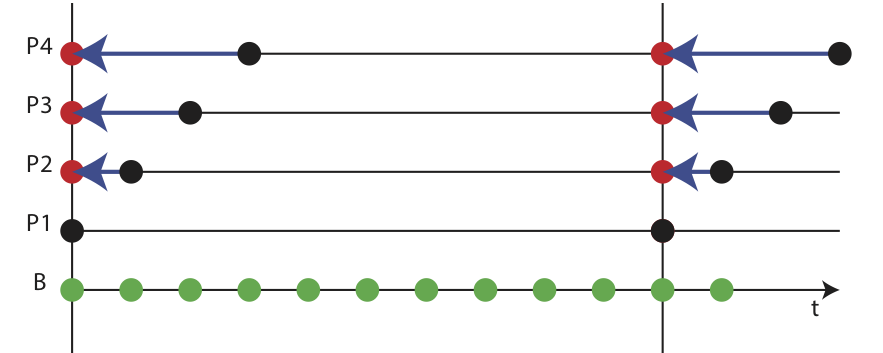
\includegraphics[width=\linewidth]{microbatches1.png}
  \caption{Microbatching logic}\label{fig:microbatch1}
\endminipage\hfill
\minipage{0.32\textwidth}
  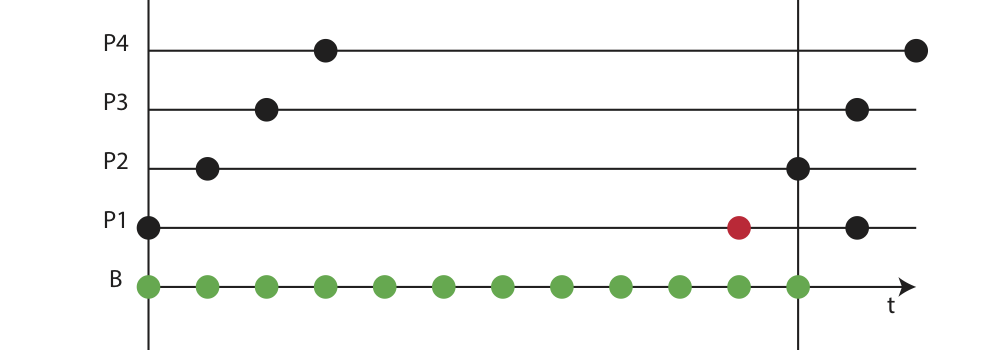
\includegraphics[width=\linewidth]{microbatches2.png}
  \caption{ Microbatching in case of misbehaving sensor}\label{fig:microbatch2}
\endminipage\hfill
\minipage{0.32\textwidth}%
  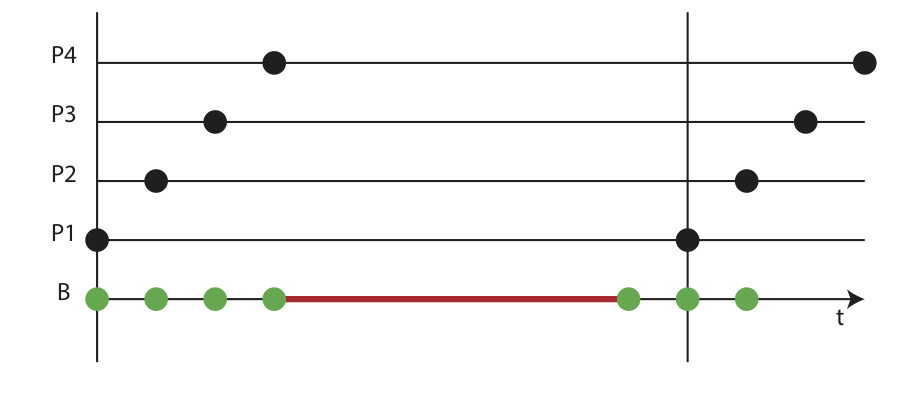
\includegraphics[width=\linewidth]{microbatches.png}
  \caption{Delta in case of missing balls}\label{fig:microbatch3}
\endminipage
\end{figure}



\IncMargin{1em}
\begin{algorithm}
\SetKwData{MicrobatchPlayers}{microbatchPlayers}\SetKwData{MicrobatchBalls}{microbatchBalls}\SetKwData{Microbatches}{microbatches}\SetKwData{NextUpdate}{nextUpdate}\SetKwData{LastBegin}{lastBegin}\SetKwData{PartialResults}{partial results}\SetKwData{Event}{event}\SetKwData{WindowNumber}{windowNumber}\SetKwData{Playing}{playing}\SetKwData{Played}{played}
\SetKwFunction{GetTypeTs}{get event type and timestamp}\SetKwFunction{ComputePossession}{compute microbatches possession}\SetKwFunction{Aggregate}{aggregate}\SetKwFunction{Print}{print}\SetKwFunction{Set}{set}\SetKwFunction{AreInside}{are inside}\SetKwFunction{IsAttached}{is attached to a }\SetKwFunction{AlreadyFound}{already found}\SetKwFunction{IsReached}{is reached}\SetKwFunction{Reset}{reset}
\SetKwInOut{Input}{input}\SetKwInOut{Output}{output}
 
 \Input{time $T$, distance $K$, full event/interruptions file $F$.}
 \Output{ball possession for both teams and single players, for both each time period $T$ and the whole game.}
 \BlankLine
    \NextUpdate $\leftarrow 1st half starting time + T$\;
    \MicrobatchPlayers$\leftarrow 0$\;
    \MicrobatchBalls$\leftarrow 0$\;
    \Microbatches$\leftarrow 0$\;
    \LastBegin$\leftarrow 0$\;
    \ForEach{\Event $\in F$}{
        \GetTypeTs\;
        \If {\Event $timestamp > \NextUpdate$}{
            \If{\Microbatches $size > 0 \ \&\& \ \MicrobatchBalls size > 0$}{
                \ComputePossession\;
                \Reset \Microbatches\;
            }
            \If{\Playing}{
                \Played $\leftarrow \Event \ timestamp - \LastBegin$\;
                \LastBegin $\leftarrow \Event \ timestamp$\;
            }
            \Aggregate \PartialResults\;
            \Print \PartialResults\;
            \NextUpdate $\leftarrow \NextUpdate + T$\;
        }
        \uIf {\Event $type$ is $referee$}{
            \Playing $\leftarrow$ (\Event $== begin$)\;
            \eIf{\Playing}{
                \LastBegin $\leftarrow \Event \ timestamp$\;
            }{
                \Played $\leftarrow \Event \ timestamp - \LastBegin$\;
            }
        
        }
        \ElseIf{\Event is a $sensor\  event \ \&\&\  \Playing$}{
            \If{\Event $cohordinates \ \AreInside \ field$}{
                \uIf{\Event $sensor \ \IsAttached player$}{
                    \If{\Event $id \ \AlreadyFound$}{
                        \Microbatches $\leftarrow$ \MicrobatchPlayers , \MicrobatchBalls\;
                        \If {$number \ of \ microbatches \ per\  task$ \IsReached}{
                            \ComputePossession\;
                            \Reset \Microbatches\;
                        }
                        \Reset \MicrobatchPlayers , \MicrobatchBalls\;
                    }
                    \MicrobatchPlayers $\leftarrow \Event \ id$
                }
                \ElseIf{\Event $id$ \IsAttached $ball$}{
                    \MicrobatchBalls $\leftarrow \Event \ id$\;
                }
            }
        }
        
    }
  \caption{Calculate possession}
\end{algorithm}

\section{Results}
The test have been made on a Google Cloud n1-highcpu-8 machine, with 8 CPUs and a 7,20GB memory (1 CPU every 0,9GB). 
Due to access to disk being the real bottleneck of this application, the improvement given from the use of OpenMP did not go other 10\%, as we can see in Figure \ref{fig:percentage}.
Given the streaming approach we have adopted the first window is printed after 4s on average, with a total computating time of 1m35s.
K and T do not influence timings.

\begin{figure}[!htb]
\minipage{0.48\textwidth}
  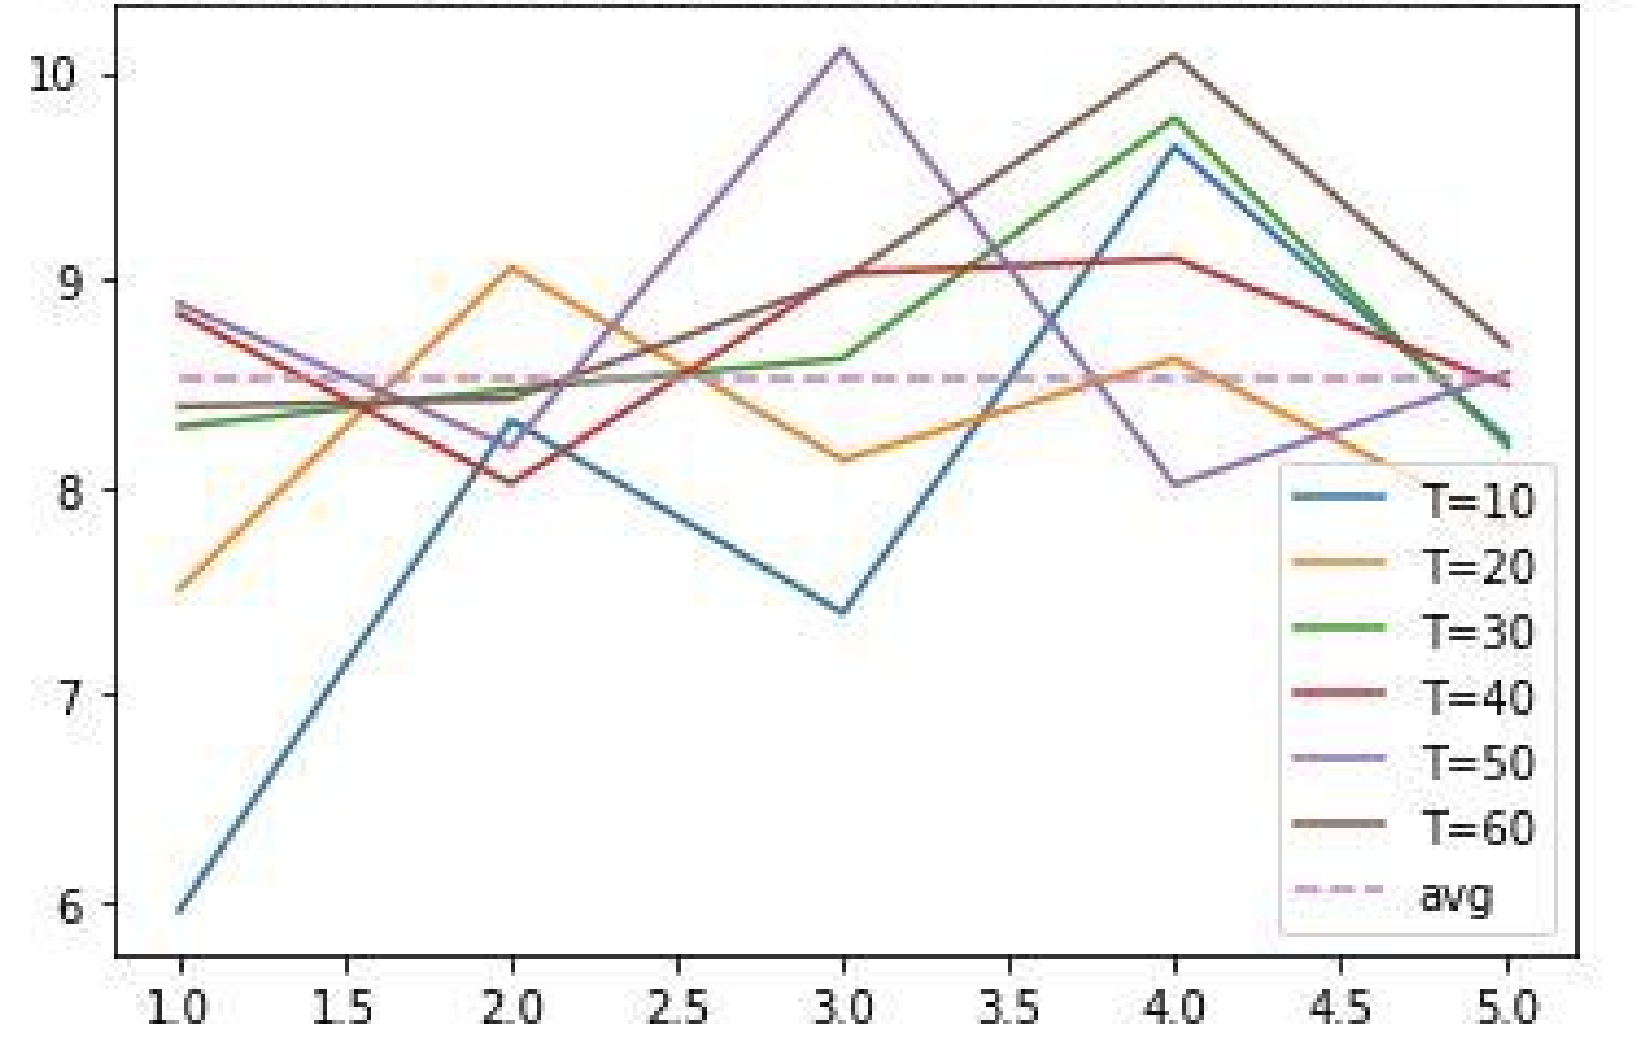
\includegraphics[width=\linewidth]{gross.png}
  \caption{Delta serial-parallel for K from 1 to 5 and T from 10 to 60}\label{fig:gross}
\endminipage\hfill
\minipage{0.48\textwidth}
  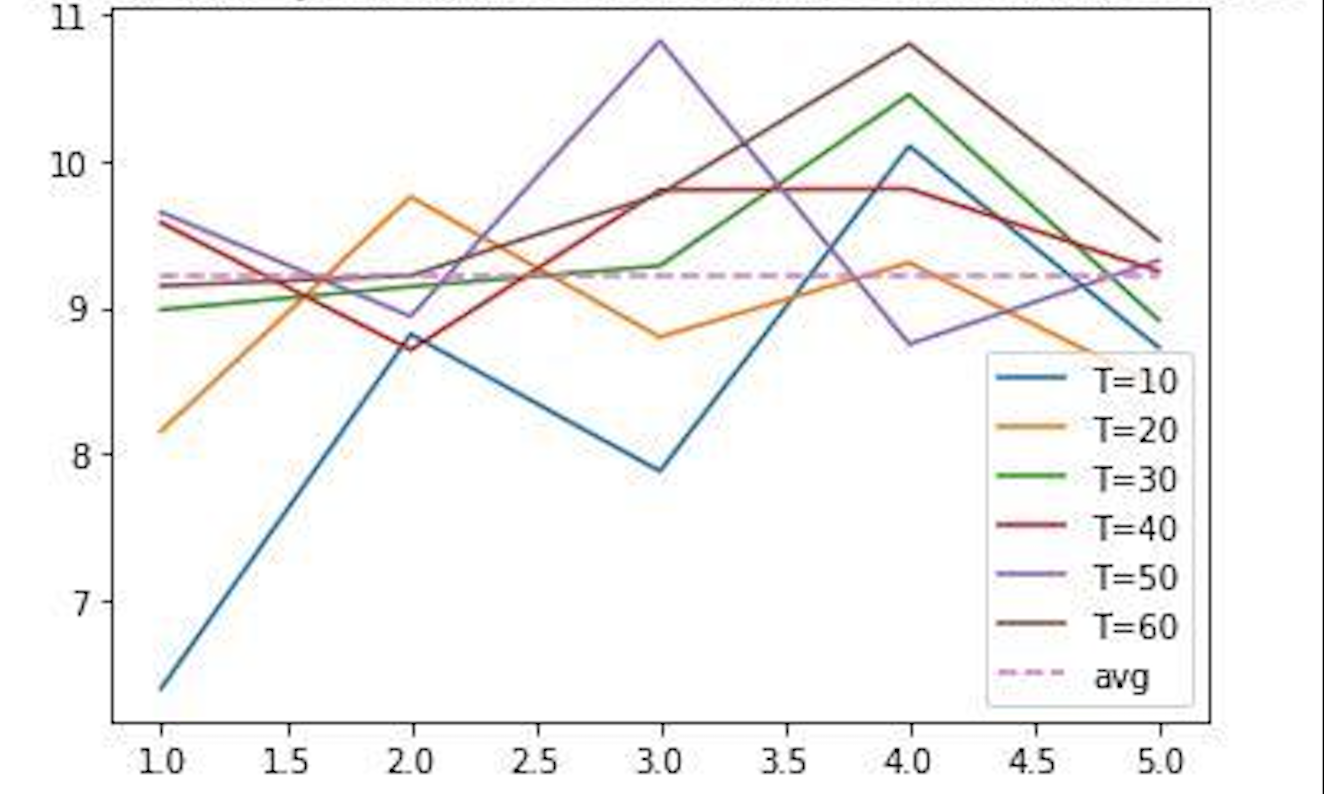
\includegraphics[width=\linewidth]{percentage.png}
  \caption{percentage Delta serial-parallel for K from 1 to 5 and T from 10 to 60\label{fig:percentage}}
\endminipage\hfill
\end{figure}
\end{document}